\section{اندازه‌گیری کارایی نرم‌افزار}

\subsection{\lr{Responsiveness} یا پاسخگویی}

در پاسخگویی مطرح می‌شود که یک تسک چقدر سریع می‌تواند توسط یک سیستم تمام شود.
معمولاً با \lr{Waiting time} و \lr{Queue length} می‌توان اندازه‌گیری کرد.

\subsection{\lr{Usage level} یا سطح استفاده}

به چه اندازه‌ای می‌توانیم به صورت مناسب و مطلوب از المان‌های مختلف در سیستممان
استفاده کنیم. معیار‌های اندازه‌گیری آن \lr{Throughput} یا گذردهی و
\lr{Utilization} می‌باشد.

\subsection{\lr{Waiting time}}

مدت زمان بین رسیدن تسک به سرویس و شروع ارائه سرویس به آن تسک (درخواست) را
می‌گویند.

\subsection{\lr{Queue length}}

تعداد تسک‌ها (درخواست‌ها) در صف انتظار برای سرویس‌گیری.

\subsection{\lr{Task length or Service time}}

به هر درخواست درون صف چقدر طول می‌کشد که سرویس‌دهی انجام شود. عموماً وابسته به
میزان پردازشی سرور و محاسبه درخواست می‌باشد.

\subsection{\lr{Utilization}}

مدت زمانی که یک قطعه از تجهیزات در حال استفاده است نسبت به کل زمان استفاده از
آن، محاسبه می‌شود.

\subsection{\lr{Throughput}}

نرخ کامل شدن تسک‌ها در سیستم می‌باشد.

\subsection{\lr{Good-put}}

داده‌ای است که باز ارسال نشده باشد. یک بسته سالم بدون هیچ باز ارسالی از سمت مبدا
به سمت مقصد را گویند.

\subsection{\lr{Missionability} یا ماموریت‌پذیری}

ماموریت‌پذیری نشان می‌دهد که سیستم مورد نظر در آن بازه زمانی که عملیاتی را انجام
می‌داده است چقدر رضایت در کارایی و گذردهی داشته است. چقدر در آن زمانی که در
دسترس بوده است تسک‌هایی را رد کرده و تسک‌هایی را با موفقیت انجام داده است.

\subsection{\lr{Dependability}}

این اندازه‌گیری مشخص می‌کند که چقدر یک سیستم در طول اجرا قابل اطمینان می‌باشد.
فرمول‌هایی را مطرح می‌کند که همگی از نوع زمان هستند. نکته آن است که تعداد
شکست‌ها در سیستم باید کم باشد و همچنین زمانی که در وضعیت شکست قرار داریم بایستی
سریع ریکاوری انجام شود تا دوباره سیستم به حالت صحیح قبلی خود بازگردد.

ابزار‌های اندازه‌گیری آن عبارت‌اند از:

\begin{itemize}
    \item \lr{Number of failures per day}
    \item \lr{MTTF (Mean Time to Failure)}
    \item \lr{MTTR (Mean Time to Recovery or Repair)}
    \item \lr{Long Term Availability}
    \item \lr{Cost of Failure}
\end{itemize}

\subsection{\lr{Productivity} یا معیار بهره‌وری}

این معیار مشخص می‌کند که یک کاربر چقدر بهینه می‌تواند کار خود را با محصول مورد
نظر انجام دهد.

ابزار‌های اندازه‌گیری آن عبارت‌اند از:

\begin{itemize}
    \item \lr{User Friendliness}
    \item \lr{Understandability}
\end{itemize}

برای مثال، \lr{User Interface (UI)} یک اپلیکیشن موبایل چقدر خوب طراحی شده است که
کاربر می‌تواند در سریع‌ترین حالت ممکن گزینه‌های مدنظر خود را پیدا کند؟

\subsection{دسترس‌پذیری، قابلیت اعتماد و قابلیت اطمینان}

\subsubsection{\lr{Mean Time Between Failures (MTBF)}}

زمان سپری شده پیشبینی شده بین خرابی‌های یک سیستم در حین کار است. \lr{MTBF}
می‌تواند زمان بین خرابی‌های یک سیستم را محاسبه کند.

\begin{LTR}
    MTBF Defined as: total time in service / number of failures
\end{LTR}

\begin{equation}
    MTBF = \frac{\sum(X - Y)}{Z}
\end{equation}

\begin{itemize}
    \item \lr{X}: \lr{Start of downtime}
    \item \lr{Y}: \lr{Start of uptime}
    \item \lr{Z}: \lr{Number of failures}
\end{itemize}

\begin{figure}[H]
    \centering
    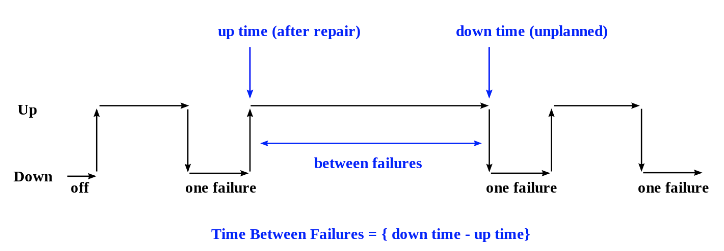
\includegraphics[width=0.9\textwidth]{images/mtbf.png}
    \caption{\lr{Mean Time Between Failures (MTBF)}}
    \label{fig:MTBFDiagram}
\end{figure}

\subsubsection{\lr{Mean Time to Failures (MTTF)}}

طول زمانی که انتظار داریم یک دستگاه یا هر چیزی در مدار باقی بماند. \lr{MTTF}
معیاری است که در سخت‌افزار استفاده می‌شود. مدت زمانی که انتظار داریم یک دستگاه
یا محصول کار کند. \lr{MTTF} یکی از هزاران راه‌یی است که می‌توان قابلیت اعتماد و
پایداری سخت‌افزار یا بقیه تکنولوژی‌ها را با آن اندازه‌گیری کرد.

\subsubsection{\lr{Mean Time to Repair or Recovery (MTTR)}}

مدت زمانی که طول می‌کشد تا سیستم به مدار برگردد. یا به عبارتی دیگر میانگین زمانی
که نیاز است تا یک کامپوننت شکست خورده تعمیر و ریکاوری شود.

\subsubsection{تفاوت میان \lr{MTTF} و \lr{MTBF}}

\begin{itemize}
    \item معیار \lr{MTBF} برای محصولاتی است که می‌توان آن‌ها را در حین خرابی
    تعمیر کرد تا سریعاً به مدار بازگردد.
    \item معیار \lr{MTTF} برای محصولاتی که قابل تعمیر نیستند استفاده می‌شود.
    زمانی از این معیار استفاده می‌کنیم که به دنبال تعمیرپذیری محصول نباشیم.
\end{itemize}

\subsection*{نکته}

\begin{itemize}
    \item بازه‌های زمانی بررسی سیستم در سازمان بایستی به صورت مشخص باشد (ساعتی،
    روزانه، هفتگی، ماهانه، سالانه).
    \item یک قطعه (دستگاه، نرم‌افزار و هر چیزی) می‌تواند \lr{Available} باشد ولی
    \lr{Reliable} نباشد.
    \item نرخ خرابی: $\frac{Number Of Failures}{Total Time In Service}$
\end{itemize}